\minitoc  % Affiche la table des matières pour ce chapitre

% ==================================================================================================================================
% Cauchy-Lipschitz

\section{Cauchy-Lipschitz}

\textbf{Problème : } On cherche une condition suffisante d'existence et d'unicité d'une solution maximale au problème 
de Cauchy: 
    \[ (P) : 
        \begin{cases}
            (E) : y'(t) = f(t,y) \\ 
            (C) : y(t_0) = y_0 
        \end{cases}
    \] 

\begin{definition}[Fonction Localement Lipschitzienne]
    Soit 
        \[ f : 
            \begin{cases}
                \Omega = I \times \Omega' \longrightarrow \K^n \\ 
                (t,x) \longmapsto f(t,x)
            \end{cases} \] 
    On dit que $f$ est LLVE (localement lipschitzienne en la variable d'état i.e $x$) \underline{si} :
        \[ \forall (t_0, y_0) \in I \times \Omega', \exists [t_0 - \alpha, t_0 + \alpha] \times B_f(y_0,r) \] 
    Tel que : 
        \[ \exists k \in \R_+, \forall t \in [t_0 - \alpha, t_0 + \alpha], \text{ on a : } \] 
        \[ \boxed{ \forall x,x' \in B_f(y_0,r), \| f(t,x) = f(t,x') \| \leqslant k \| x - x'\| } \] 
    
    \emph{On cherche donc un cylindre $[t_0 - \alpha, t_0 + \alpha] \times B_f(y_0,r) \subset I \times \Omega'$ sur lequel 
    $f$ soit lipschitzienne.}
\end{definition}

\begin{comment}
    \begin{center}
        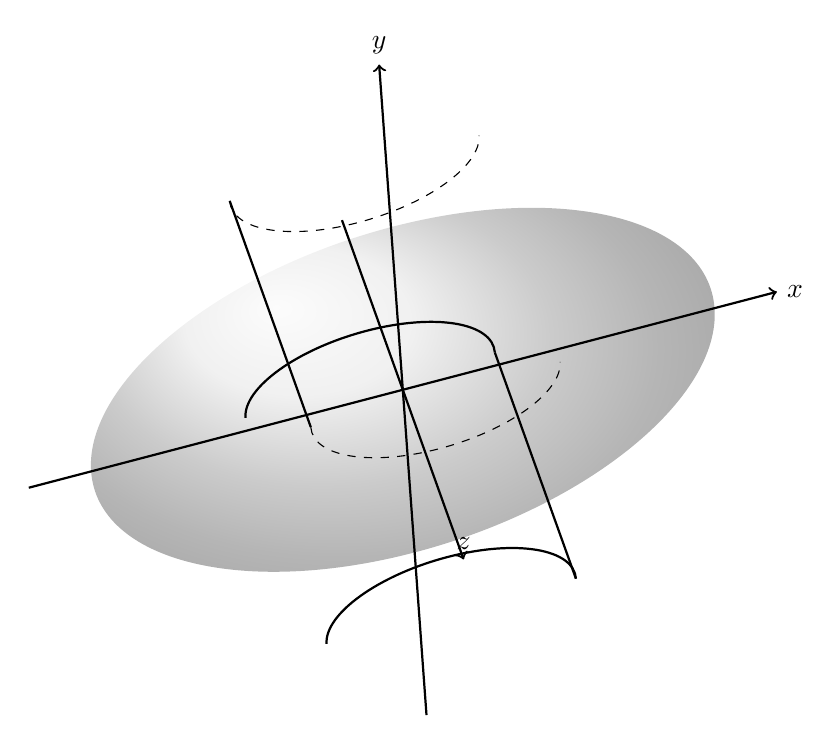
\begin{tikzpicture}
    
            % Définition de la perspective
            \begin{scope}[scale=1.5, rotate around x=10, rotate around y=30]
        
                % Boule irrégulière (ellipsoïde en 3D)
                \shade[ball color=gray!30, opacity=0.5] (0,0,0) ellipse (2.5 and 1.5);
        
                % Cylindre : bases et côtés
                \draw[thick] (1,-1,-2) -- (1,-1,2);
                \draw[thick] (-1,1,-2) -- (-1,1,2);
                
                % Dessin des bases du cylindre
                \draw[thick] (1,-1,2) arc[start angle=0, end angle=180, x radius=1, y radius=0.5];
                \draw[dashed] (-1,1,2) arc[start angle=180, end angle=360, x radius=1, y radius=0.5];
                
                \draw[thick] (1,-1,-2) arc[start angle=0, end angle=180, x radius=1, y radius=0.5];
                \draw[dashed] (-1,1,-2) arc[start angle=180, end angle=360, x radius=1, y radius=0.5];
        
                % Axes orthonormés
                \draw[thick,->] (-3,0,0) -- (3,0,0) node[right] {$x$};
                \draw[thick,->] (0,-3,0) -- (0,3,0) node[above] {$y$};
                \draw[thick,->] (0,0,-3) -- (0,0,3) node[above] {$z$};
        
            \end{scope}
        
        \end{tikzpicture}
    \end{center}
\end{comment}

\begin{definition}[Fonction Lipschitzienne en la variable d'état]
    Soit 
    \[ f : 
        \begin{cases}
            \Omega = I \times \Omega' \longrightarrow \K^n \\ 
            (t,x) \longmapsto f(t,x)
        \end{cases} \] 
    On dit que $f$ est LVE (lipschitzienne en la variable d'état i.e $x$) \underline{si} :
    \[ \forall J \in I \text{ compact } \exists k \in \R_+ \text{ tel que } : \] 
    \[ \forall t \in J, \forall x, x' \in \Omega', \quad \boxed{\| f(t,x) - f(t,x')\| \leqslant k \| x - x' \| } \]  
\end{definition}

\begin{remark}
    Une fonction lipschitzienne en la variable d'état est localement lipschitzienne en la variable d'état. 
    \[ \text{i.e} \quad LVE \Longrightarrow LLVE \] 
\end{remark}

\begin{example}
    Soit $f : (t,x) \longmapsto A(t)x + B(t)$. Supposons que $A, B \in \mathcal{C}^0(I, \mathcal{M}_n(\K))$.

    $f$ est LVE car $ \forall t \in J, x,x' \in \K^n$ où $J \subset I$, on a : 
        \begin{align*}
            \| f(t,x) - f(t,x') \| &= \| A(t) (x-x') \| \\ 
            & \leqslant \| A(t)\| \times \| x-x'\| \\ 
            & \leqslant \sup_{t \in J} \| A(t) \| \in \R_+ 
        \end{align*}
\end{example}

\begin{theorem}[Cauchy-Lipschitz LVE]
    Soit 
        \[ (P) : 
            \begin{cases}
                (E) : y'(t) = f(t,y) \\ 
                (C) : y(t_0) = y_0
            \end{cases} 
        \quad \text{où } f : I \times \Omega \overset{\text{LVE}}{\longrightarrow} \K^n \] 
    \underline{Alors} il existe une unique solution maximale au problème de Cauchy $(P)$. 
    Cette solution est même globale. 
\end{theorem}

\begin{theorem}[Cauchy-Lipschitz LLVE]
    Soit 
        \[ (P) : 
            \begin{cases}
                (E) : y'(t) = f(t,y) \\ 
                (C) : y(t_0) = y_0
            \end{cases} 
        \quad \text{où } f : I \times \Omega \overset{\text{LLVE}}{\longrightarrow} \K^n \] 
    \underline{Alors} il existe une unique solution \textbf{maximale} au problème de Cauchy $(P)$. 
\end{theorem}

\textbf{Attention : } Cette solution n'est pas forcément globale. 

\begin{example}
    \[ f : 
        \begin{cases}
            \R \times \R \longrightarrow \R \\ 
            (t,x) \longmapsto x^2
        \end{cases} 
        \quad \text{LLVE mais non LVE} 
        \quad  g : 
        \begin{cases}
            R \times R \longrightarrow \R \\ 
            (t,x) \longmapsto \sqrt{|x|}
        \end{cases}
        \quad \mathcal{C}^0 \text{ mais pas LLVE} \] 
\end{example}

En pratique nous utiliserons plutôt le résultat suivant pour invoquer le théorème de Cauchy-Lipschitz. 

\begin{proposition}
    Toute fonction $ \mathcal{C}^1$ par rapport à la variable d'état est LLVE. 
\end{proposition}


% ==================================================================================================================================
% Equations à variables séparables

\newpage

\section{Équations à variables séparables}

\begin{definition}[Équation différentielle à variable séparable]
    Une équation différentielle à variables séparables est une équation différentielle scalaire de la forme : 
        \[ (E) : y'(t) = f(y)g(t) \] 
    où : 
    \begin{itemize}
        \item $f : \Omega \overset{ \mathcal{C}^0}{\longrightarrow} \K $
        \item $g : I \overset{ \mathcal{C}^0}{\longrightarrow} \K $ 
    \end{itemize}
\end{definition}

\begin{example}
    Quelques exemples d'équation différentielles à variables séparables : 

\end{example}


% ==================================================================================================================================
% Théorème de sortie de tout compact

\section{Théorème de sortie de tout compact}

\begin{theorem}[Sortie de tout compact]
    Soit $(E) : y'(t) = f(t,y)$ sur $]a,b[$ où : 
        \[ f : ]a,b[ \times \Omega \longrightarrow \K^n \] 
    Soit $y : ]c,d[ \longrightarrow \K^n$ une solution maximale de $(E)$ non globale telle que $d < b$. 

    \underline{Alors} $ \forall K \subseteq \Omega$ compact, il existe un voisinnage $V$ de $d$ tel que : 
        \[ \forall t \in V, y(t) \not \in K \] 
\end{theorem}

\begin{comment}
    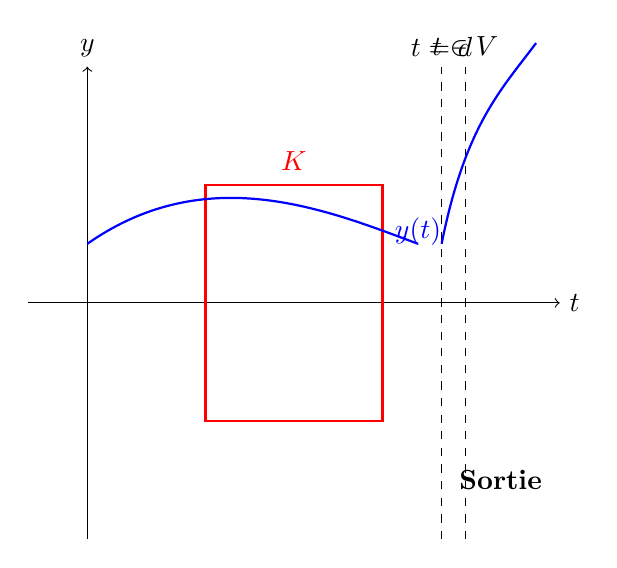
\begin{tikzpicture}[scale=1.5]
        % Axes
        \draw[->] (-0.5,0) -- (4,0) node[right] {$t$};
        \draw[->] (0,-2) -- (0,2) node[above] {$y$};
        
        % Domaine d'existence
        \draw[dashed] (3,-2) -- (3,2) node[above] {$t=d$};
        
        % Compact K
        \draw[thick, red] (1, -1) rectangle (2.5, 1);
        \node[red] at (1.75,1.2) {$K$};
        
        % Solution y(t)
        \draw[thick, blue] (0,0.5) .. controls (1,1.2) and (2,0.8) .. (2.8,0.5);
        \node[blue] at (2.8,0.6) {$y(t)$};
        
        % Zone après d
        \draw[dashed] (3.2,-2) -- (3.2,2) node[above] {$t \in V$};
        
        % Sortie du compact
        \draw[thick, blue] (3,0.5) .. controls (3.2,1.5) and (3.5,1.8) .. (3.8,2.2);
        \node at (3.5,-1.5) {\textbf{Sortie}};
    \end{tikzpicture}
\end{comment}

\begin{theorem}[Explosion]
    Avec les mêmes hypothèses et $\Omega = \K^n$, on a : 
    \begin{itemize}
        \item Si $b > d$ alors $ \| y(t) \| \underset{t \to d}{\longrightarrow} \infty $ 
            \begin{quote}
                Par contraposée, si $ \| y(t) \| \underset{t \to d}{ \not \longrightarrow} \infty $ 
                (i.e $y$ est bornée au voisinnage de $d$) alors $b = d$
            \end{quote}
        \item Si $y$ est bornée alors elle est globale. 
        \item Si $f$ est bornée alors toute fonction maximale est globale. 
    \end{itemize}
\end{theorem}


% ==================================================================================================================================
% Flot d'unt équation différentielle

\section{Flot d'une équation différentielle}

\begin{definition}[Flot]
    Soit $(E) : y'(t) = f(t,y)$ où 
        \[ f : \Omega \subset \R \times \K^n \longrightarrow \K^n \quad \text{LLVE} \] 
    Le flot de cette équation est la fonction : 
        \[ \Phi : 
            \begin{cases}
                D \longrightarrow \K^n \\ 
                (t,t_0, y_0) \longmapsto y_{t_0, y_0}(t) 
            \end{cases} \] 
    où 
    \begin{itemize}
        \item $y_{t_0, y_0}$ est l'unique solution maximale de $(E)$ qui vérifie $y(t_0) = y_0$. 
        \item $D = \{(t,t_0, y_0) \; | \; t \in I_{t_0, y_0}\} $
        \item $I_{t_0, y_0}$ est le domaine de définition de $t_0$ et $y_0$
    \end{itemize}
\end{definition}

\begin{prop}[Flot]
    \begin{itemize}
        \item $D$ est un ouvert 
        \item $\Phi$ est localement lipschitzienne (et donc $ \mathcal{C}^0$)
        \item Si $f$ est $ \mathcal{C}^p$ alors $\Phi$ est $ \mathcal{C}^p$. 
    \end{itemize}
\end{prop}

\begin{definition}[Equation Différentielle à paramètre]
    Une équation différentielle à paramètre est une famille d'équation différentielles 
        \[ (E_\lambda) \; \text{où} \; E_\lambda : y'(t) = f(t,y) \] 
        \[ \text{et } \;  f : 
            \begin{cases}
                \Omega \times \Lambda \longrightarrow \K^n \\ 
                (t,x,\lambda) \longmapsto f(t,x,\lambda)
            \end{cases} \] 
\end{definition}

\begin{definition}[Flot d'une équation différentielle à paramètre]
    Soit $(E_\lambda)$ une famille d'équation différentielles à parmaètre telle que $ \forall \lambda \in \Lambda$ 
    on ait :
        \[ f(.,.,\lambda) \; \text{LLVE} \] 
    Le flot paramétré est : 
        \[ \Phi : 
            \begin{cases}
                D \longrightarrow \K^n \\ 
                (t,t_0,y_0,\lambda) \longmapsto y_{t_0, y_0, \lambda}(t) 
            \end{cases} \] 
    où $y_{t_0, y_0, \lambda}$ est l'unique solution maximale de $(E_\lambda)$ telle que $y(t_0) = y_0$. 
\end{definition}

\begin{prop}[Flot]
    \begin{itemize}
        \item $D$ est un ouvert 
        \item $\Phi$ est localement lipschitzienne (et donc $ \mathcal{C}^0$)
        \item Si $f$ est $ \mathcal{C}^p$ alors $\Phi$ est $ \mathcal{C}^p$. 
    \end{itemize}
\end{prop}